\documentclass[a4paper,11pt]{article}

% set length of paper. put 'true' before unit like 31mm = 30truemm.
\usepackage[top=25truemm,bottom=25truemm,left=23truemm,right=23truemm]{geometry}
% set font to 'Times'
\usepackage{times}
% multi column
\usepackage{multicol}
\usepackage{color}
\usepackage[dvipdfmx]{graphics}
\usepackage{amsmath,amssymb}
\usepackage{bm} % italic bold (vector)
\usepackage{authblk} % author
\usepackage{fancyhdr} % header and footer
\usepackage{graphicx}
\usepackage{ascmac}
\usepackage{caption}
\usepackage{tikz}
\usepackage{here}
\usepackage{wrapfig} % 画像にテキストを回り込ませる
\usepackage{listings} % source code
\usepackage[version=3]{mhchem} %chemical equatio
\usepackage{titlesec} % relates to section

% settings of section and subsection
%\makeatletter
%\def\section{\@startsection {section}{1}{\z@}{0.1ex plus 2ex minus -.2ex}{0.1ex plus .2ex}{\normalsize\textbf}}
%\def\subsection{\@startsection {subsection}{1}{\z@}{0.1ex plus 2ex minus -.2ex}{0.1ex plus .2ex}{\normalsize\textbf}}
%\makeatother
%\pagestyle{empty}
%
%\setlength{\textwidth}{\fullwidth}
%\setlength{\texthight}{40\baselineskip}
%\addtolength{\texthight}{\topskip}
%\setlength{voffset}{-0.55in}
%
% キャプションの設定
\captionsetup[figure]{format=plain, labelformat=simple, labelsep=space, font=footnotesize}
\captionsetup[table]{format=plain, labelformat=simple, labelsep=space, font=footnotesize}
\renewcommand{\figurename}{Figure}
\renewcommand{\tablename}{Table}
%
% setting of source code
\lstset{
    basicstyle={\scriptsize\ttfamily},
    breakindent = 30pt,
    stringstyle={\scriptsize\ttfamily},
    basicstyle={\ttfamily},
  identifierstyle={\small},
  commentstyle={\smallitshape},
  keywordstyle={\small\bfseries},
  ndkeywordstyle={\small},
  stringstyle={\small\ttfamily},
  frame={tb},
  breaklines=true,
  columns=[l]{fullflexible},
  numbers=left,
  xrightmargin=0zw,
  xleftmargin=3zw,
  numberstyle={\scriptsize},
  stepnumber=1,
  numbersep=1zw,
  keepspaces=true,
  lineskip=-0.5ex,
}
% document
\begin{document}
% START DOCUMENT
%
% HEADER
\begin{center}
  % title, author
  {\fontsize{16pt}{16pt}\selectfont Numerical Analysis assignment No. 4\\}
  \vspace{16pt}
  \fontsize{10.5pt}{12pt}\selectfont
  B6TB1505 Daichi HAYASHI (Ohnishi Lab.)\\
  \vspace{10.5pt}
  Oct. 31st, 2019.\\
  \vspace{-2mm}
\end{center}

\section{Assignment 1}
I set:
\begin{align*}
    \alpha &= 0.5 \\
    \beta &= -0.5 \\
    \gamma &= 0.02 \\
    F &= 0.0008 \\
    \omega &= 1.48
\end{align*}
The result is shown below as Figure 1.

\begin{figure}[H]
	\centering
	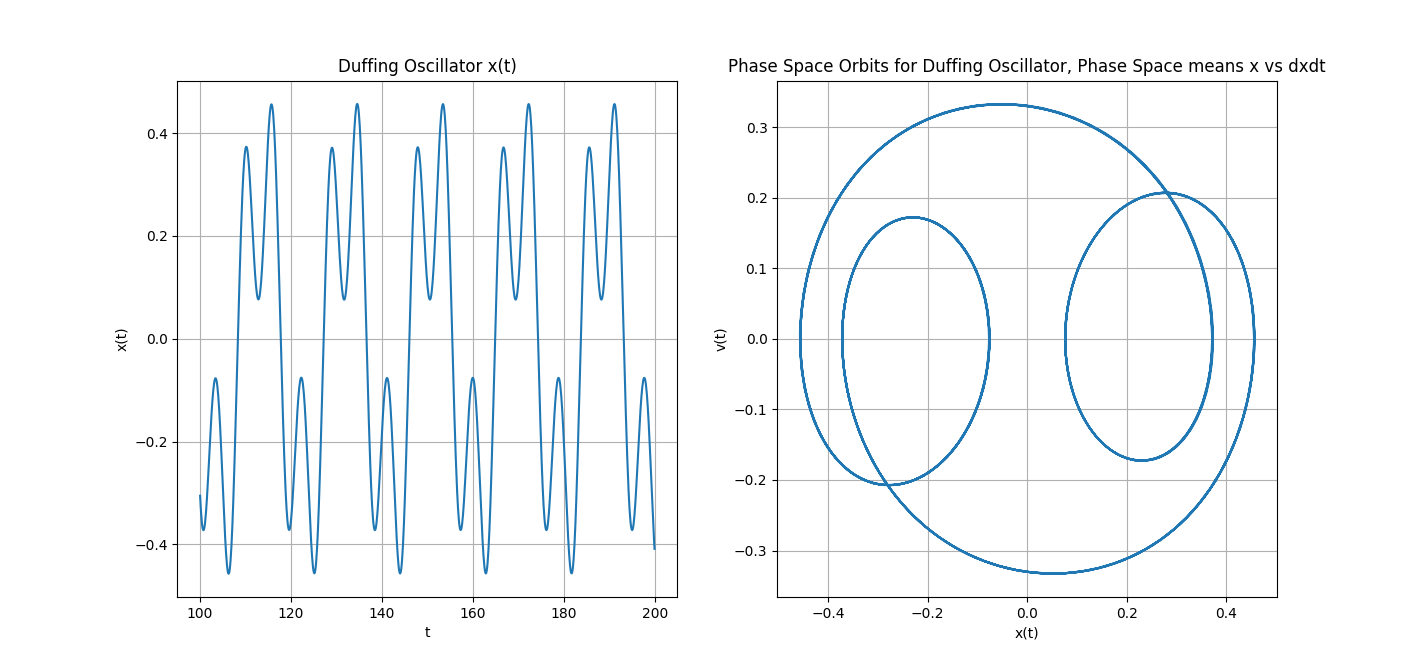
\includegraphics[width=15cm]{1.png}
	\caption{Duffing oscillator of assignment 1.} 
\end{figure}

\section{Assignment 2}
First, to express Ueda oscillator, I set $\alpha = 0$, $\beta = 1$. Then, I tested a lot of parameters to emulate the assignment figure. Finally, I set:
\begin{align*}
    \gamma &= 0.03 \\
    F &= 3.00 \\
    \omega &= 1.48
\end{align*}
The result is shown below as Figure 2.

\begin{figure}[H]
	\centering
	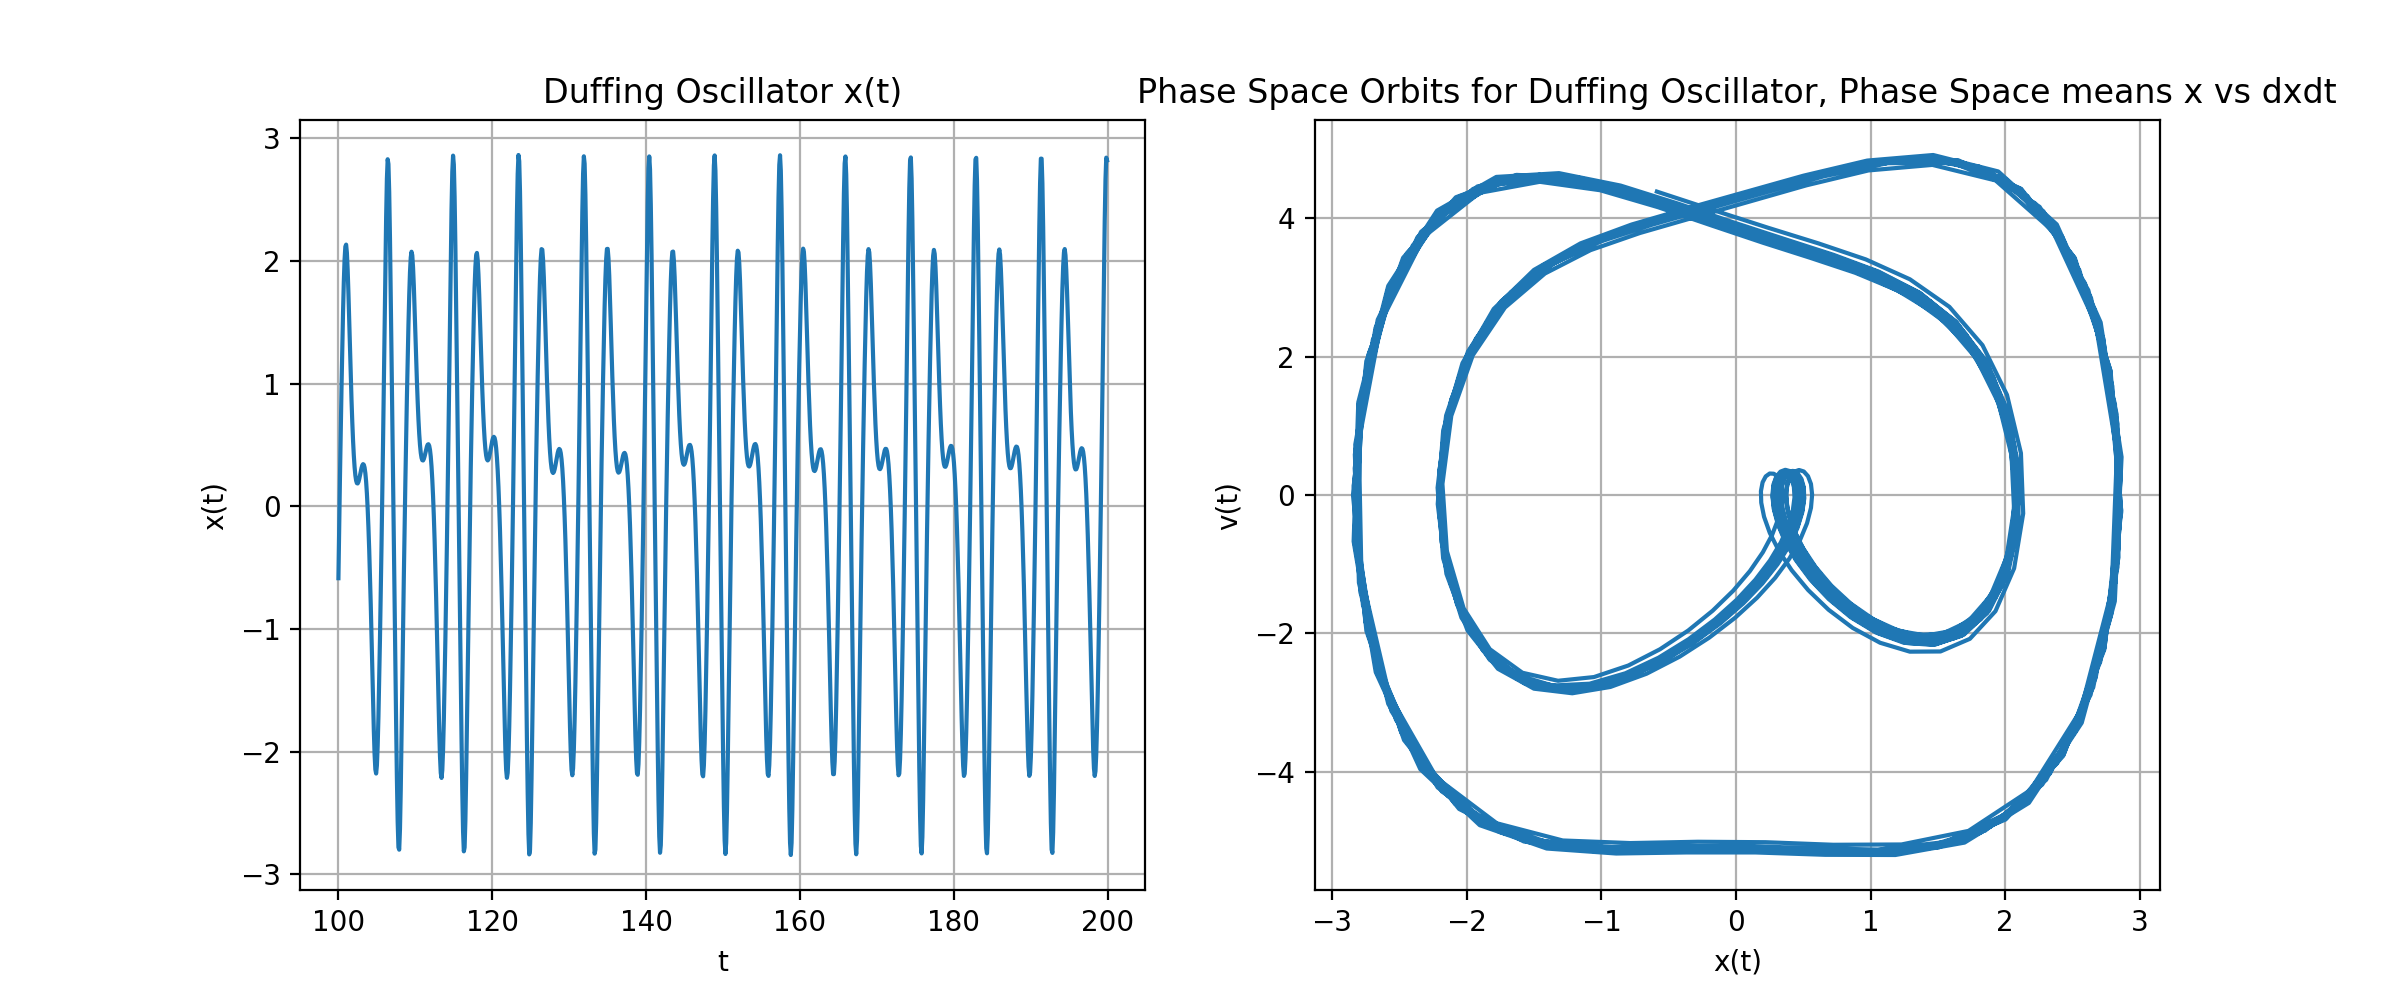
\includegraphics[width=15cm]{2.png}
	\caption{Ueda oscillator (1).} 
\end{figure}

Additionally, in the ref. [1], the parameters are:
\begin{align*}
    \gamma &= 0.01 \\
    F &= 0.9 \\
    \omega &= 1
\end{align*}
The result is shown below as Figure 2.

\begin{figure}[H]
	\centering
	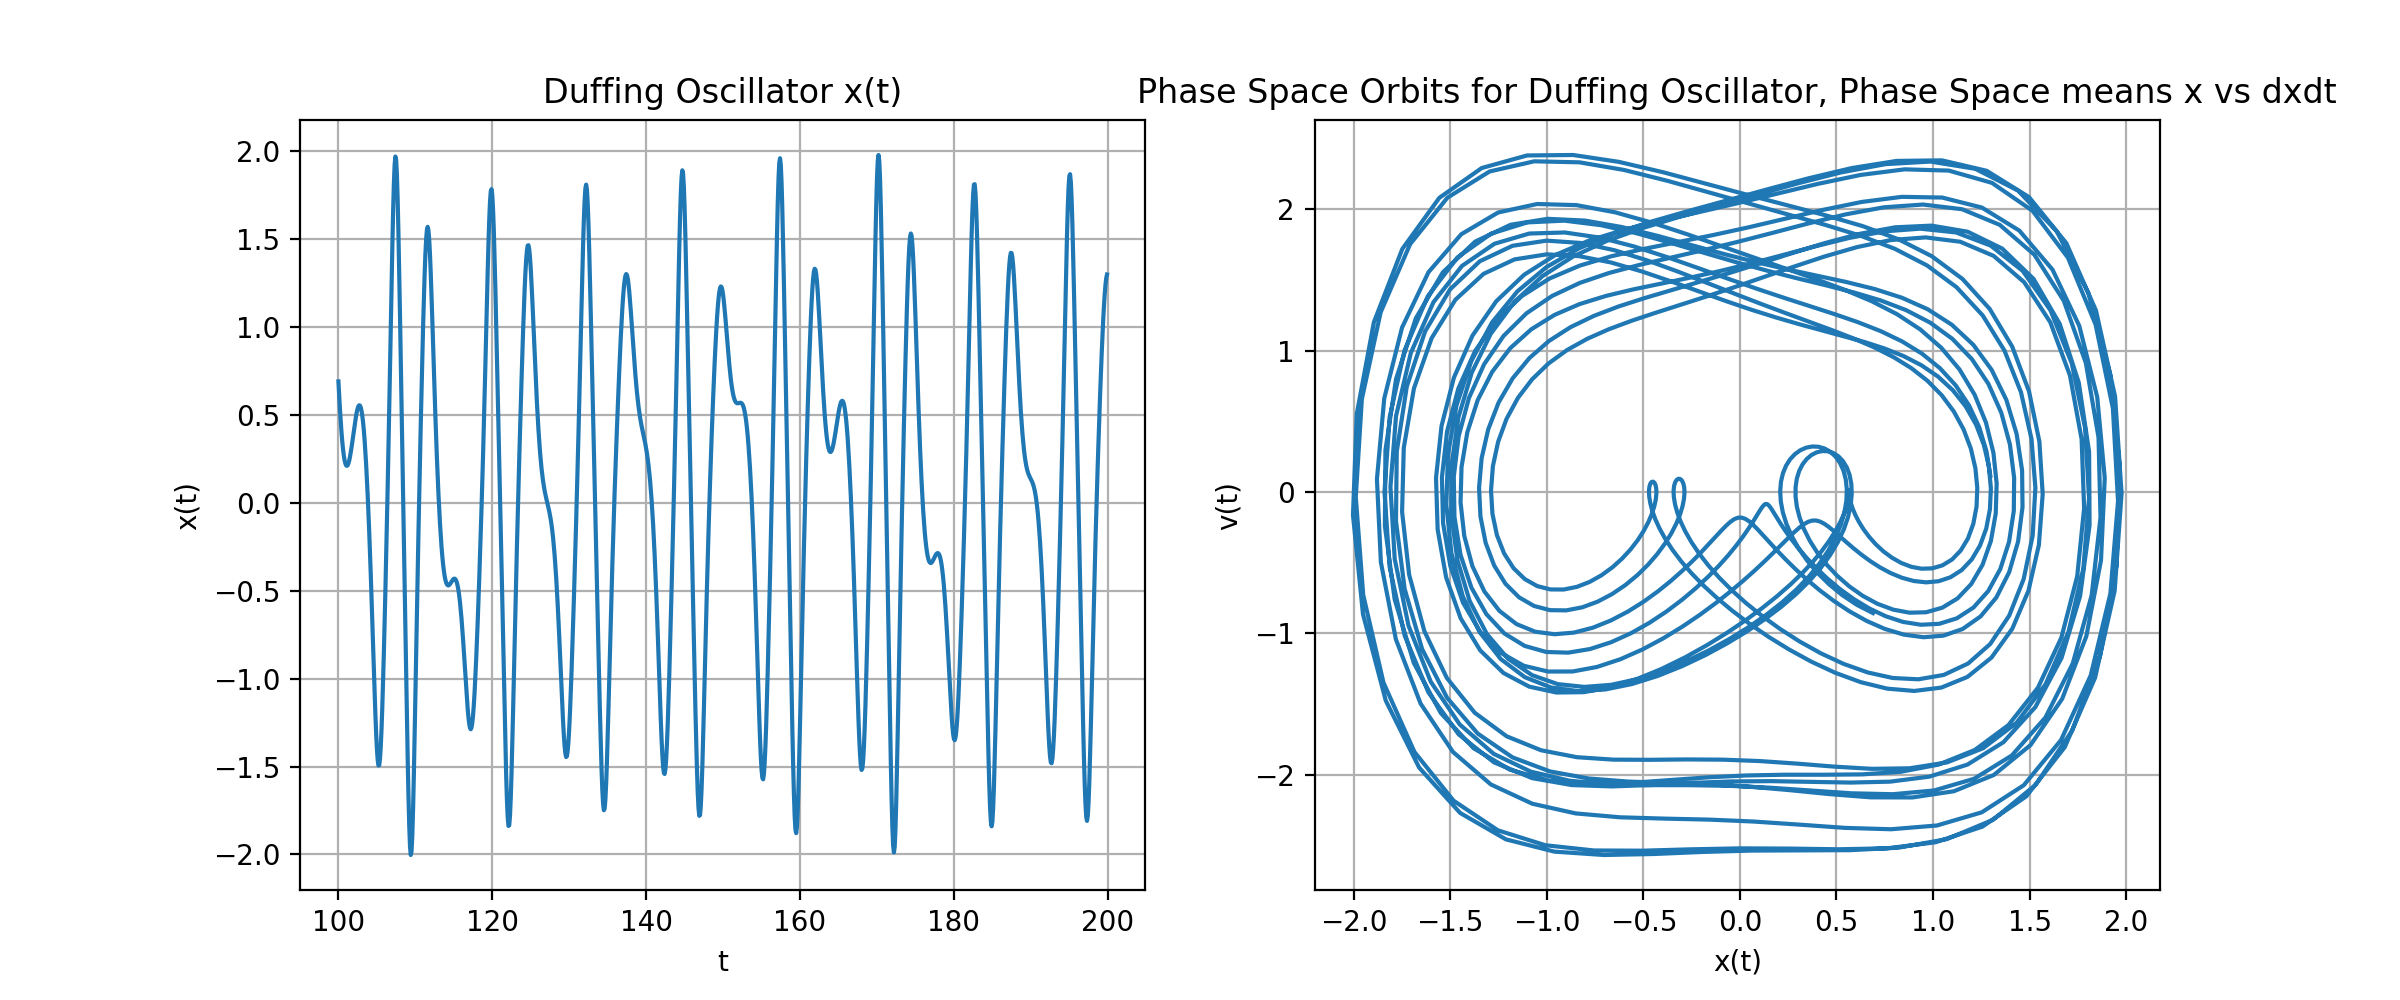
\includegraphics[width=15cm]{3.png}
	\caption{Ueda oscillator (2).} 
\end{figure}

The Ueda oscillator seems to be chaotic oscillator because when I changed one parameter a little bit (like 0.0001), the result phase space changed significantly.

\begin{thebibliography}{99}
    \bibitem{ref1}K. Ivana, B. Michael, ``\textit{The Duffing Equation: Nonlinear Oscillators and their Behaviour}'', John Wiley & Sons, 2011.
\end{thebibliography}


%
% END OF DOCUMENT
\end{document}
